\documentclass[t, 11pt]{beamer}
%% \begin{center}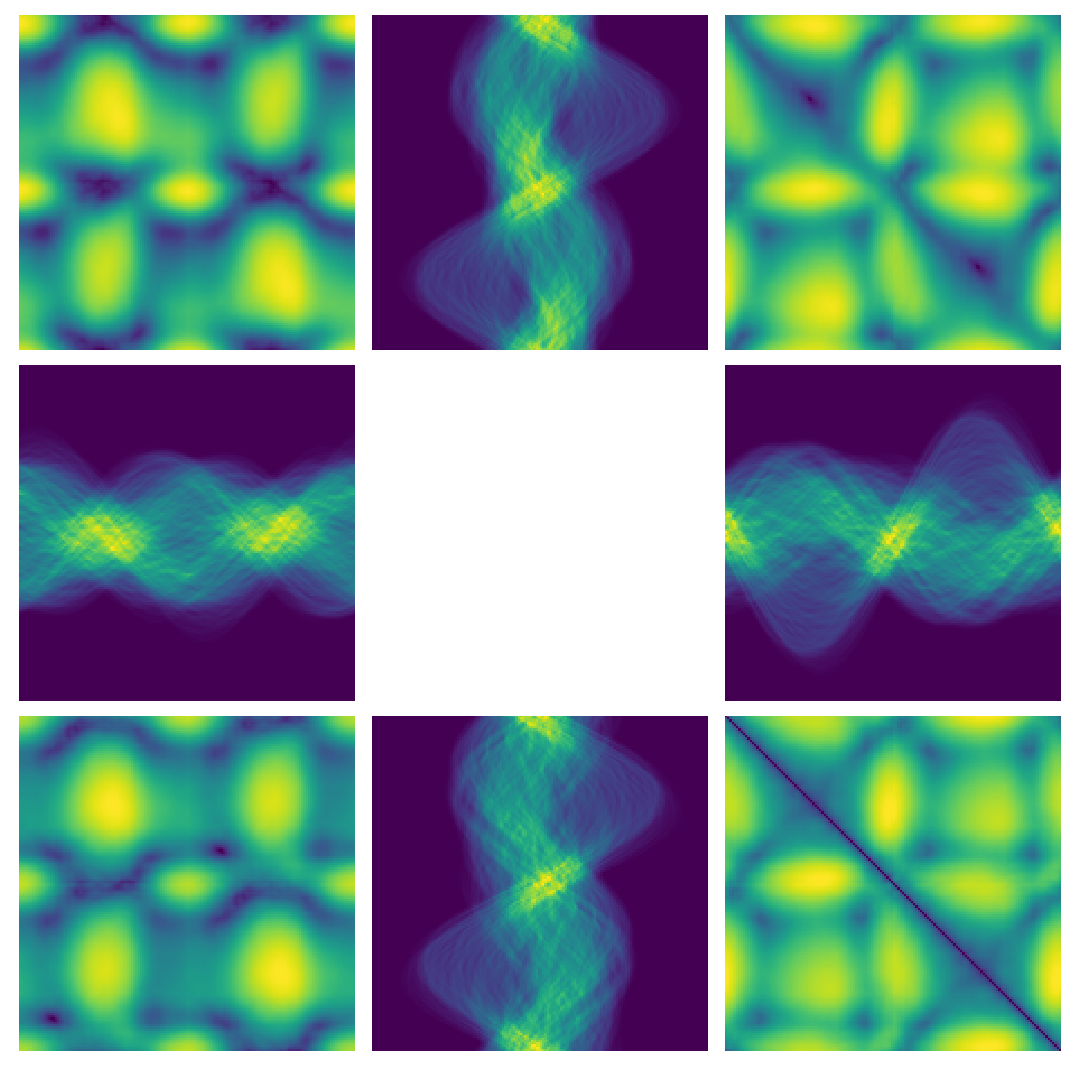
\includegraphics[width=0.45\textwidth]{images/Sinogram_3_comp.png}
%% \end{center}

\begin{document}

\small
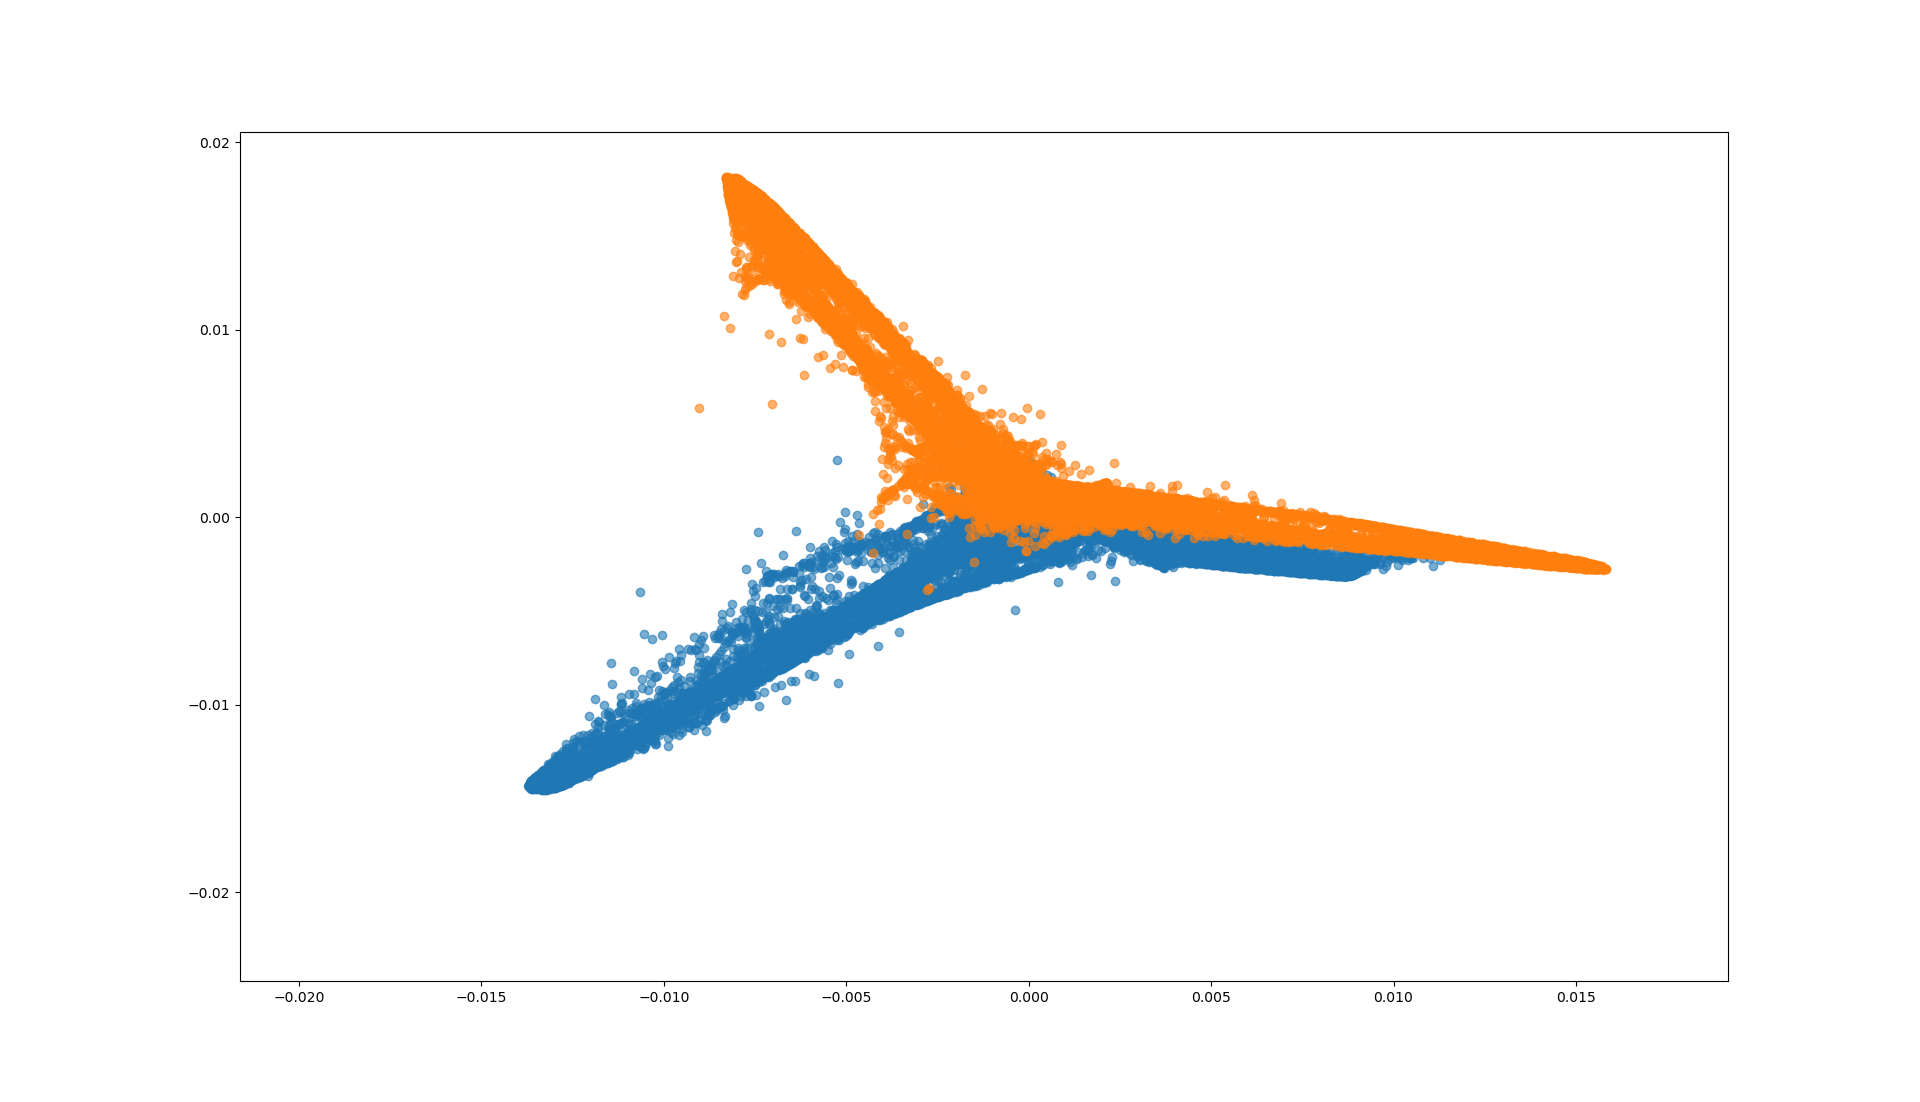
\includegraphics[width=0.60\textwidth]{../LLE_400_mixed_snr1.png} \\
SINGLELINES: LLE Dimensional reduction. 2 classes, full protein and missing medium subunit. With SNR of 1

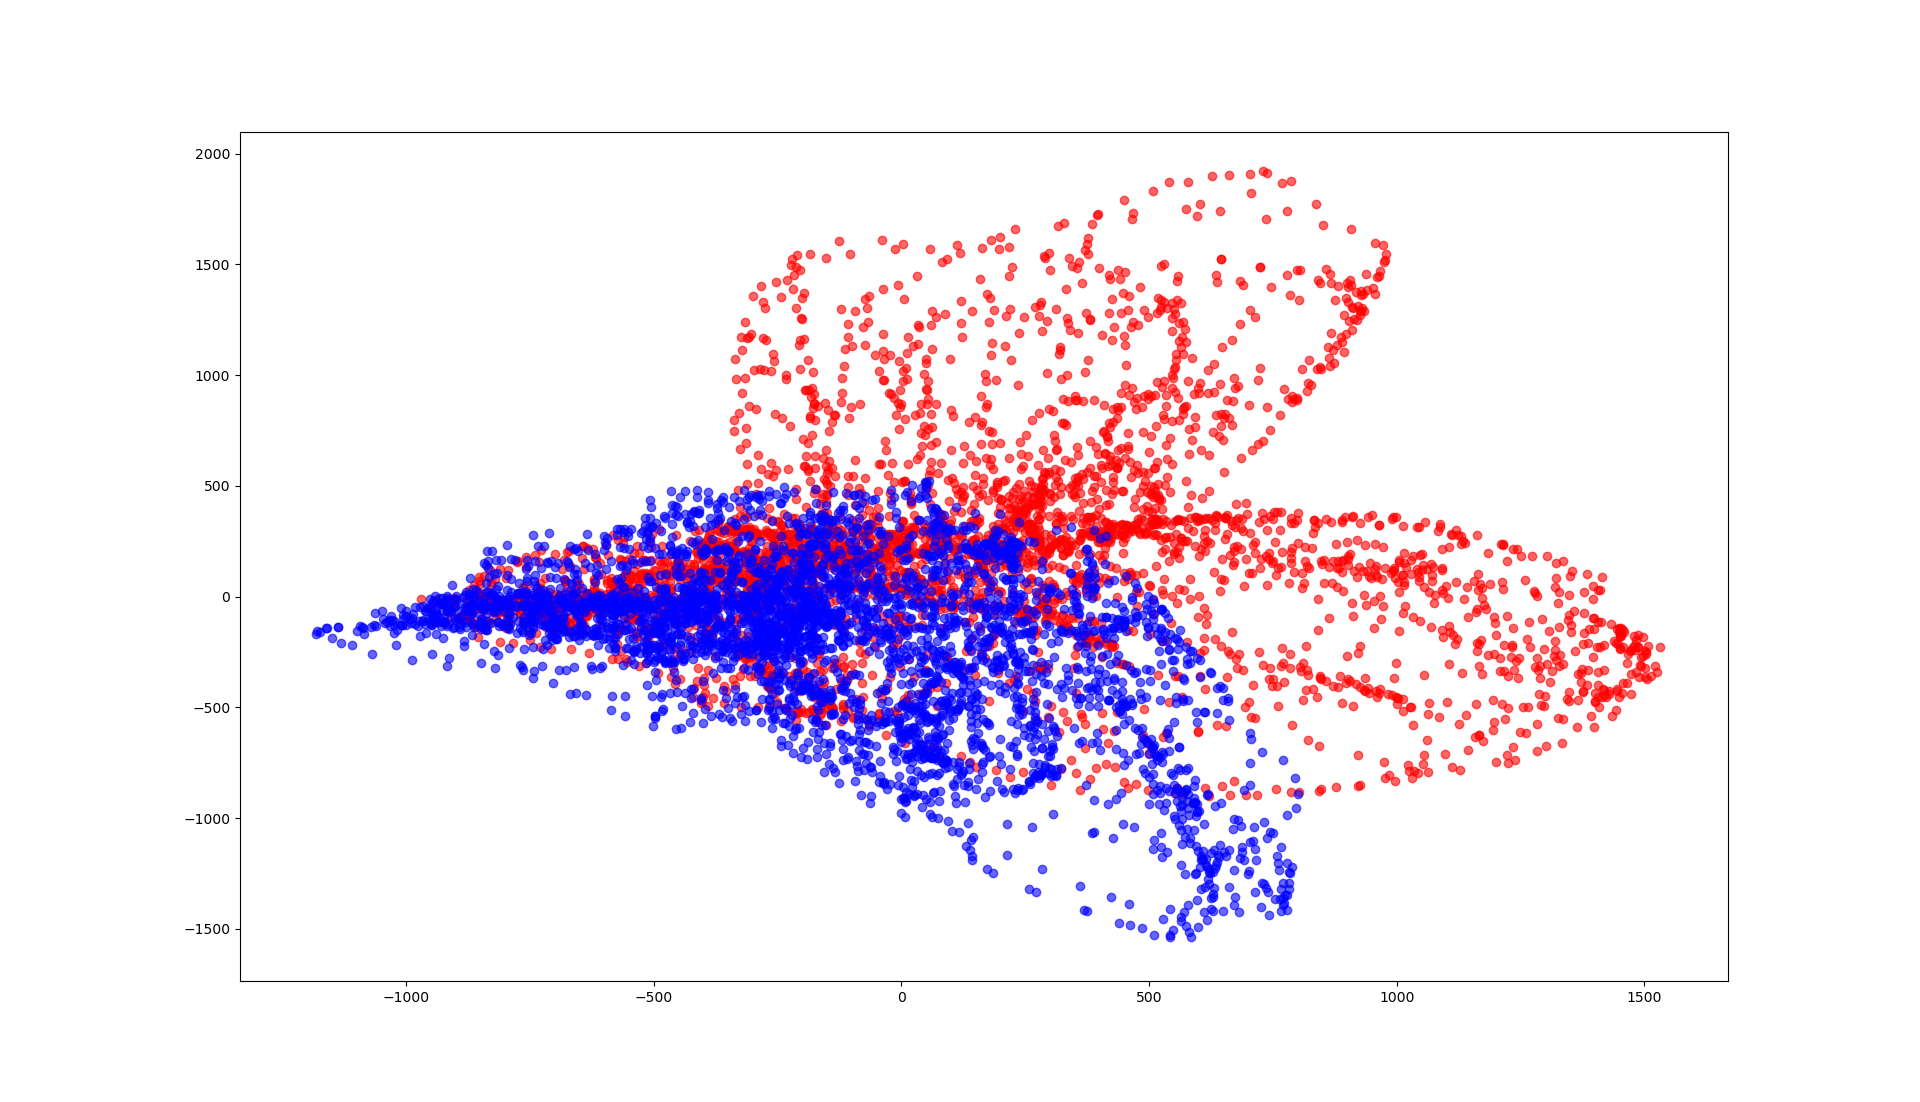
\includegraphics[width=0.60\textwidth]{../Isomap_200_mixed_snr0.png} \\
SINGLELINES: Isomap of same 2 classes. SNR 0

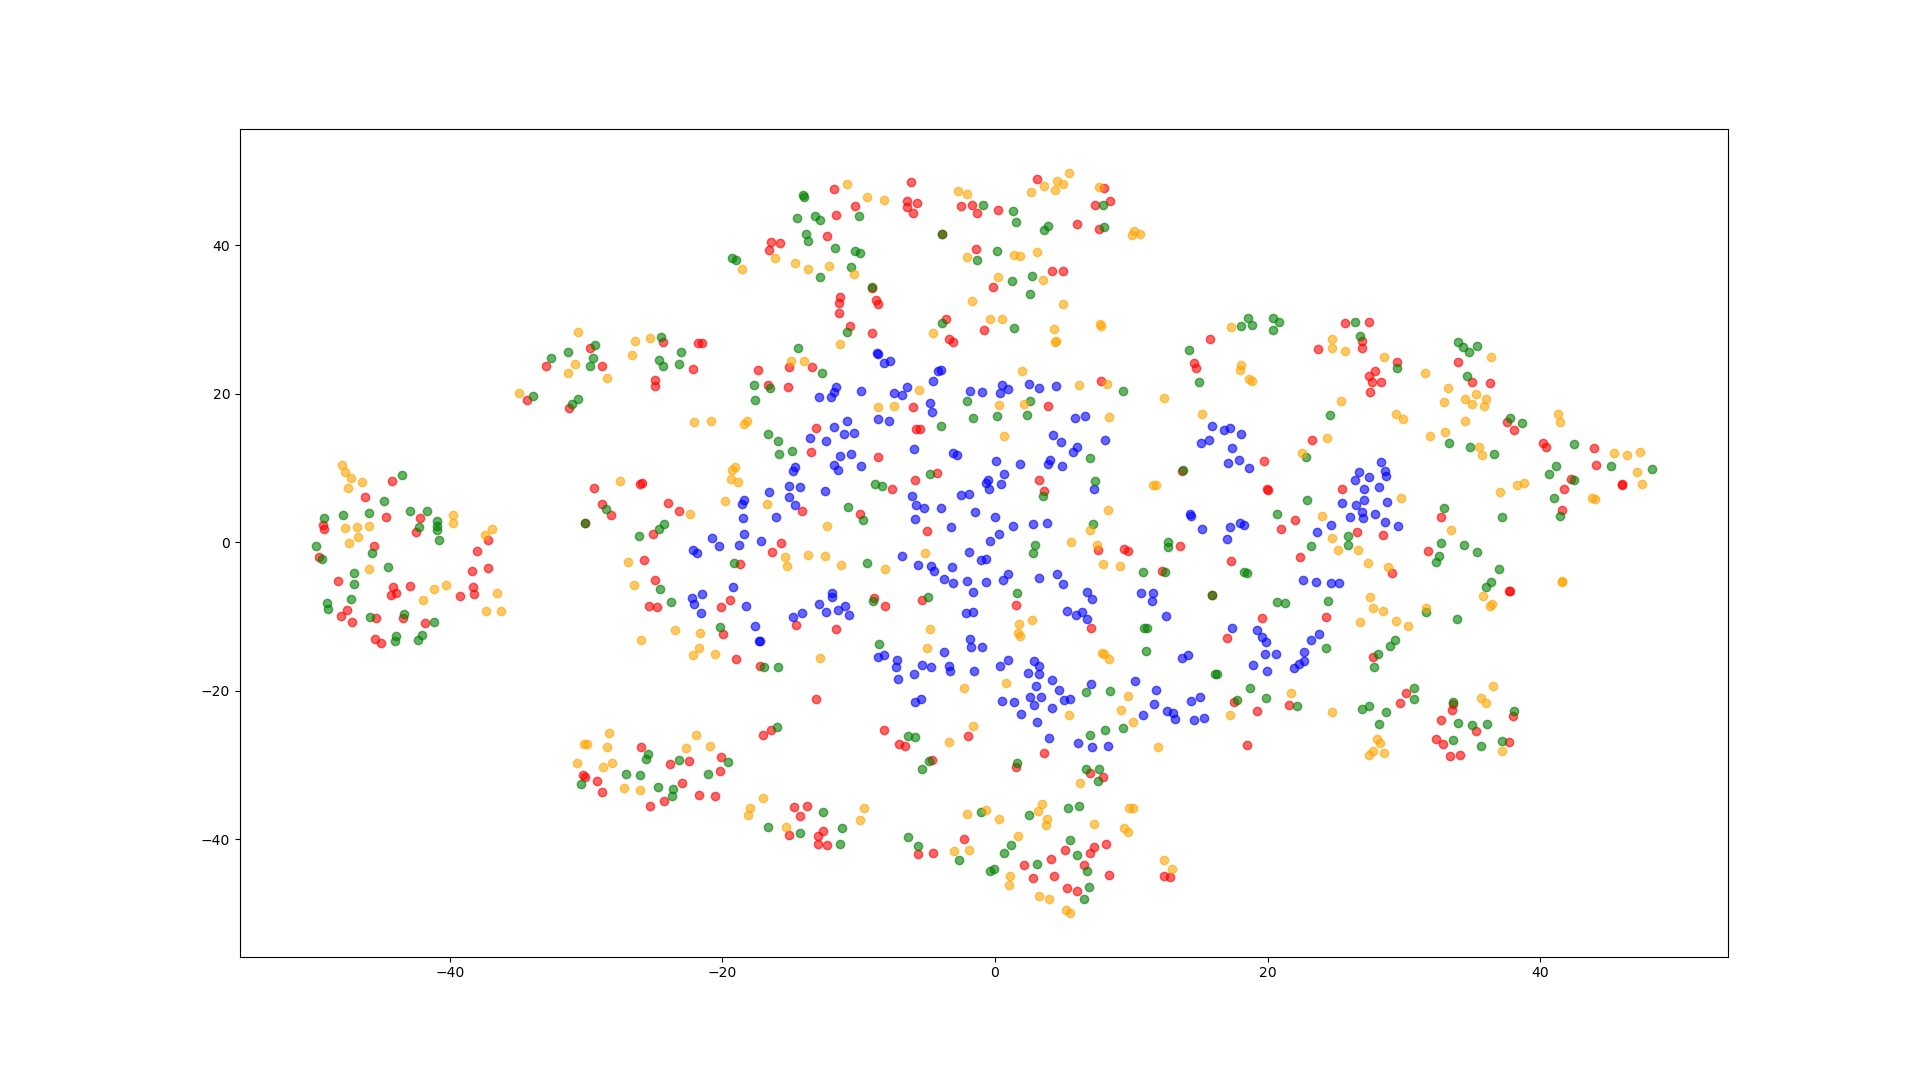
\includegraphics[width=0.60\textwidth]{../1000_TSNE_4classes_full_sinograms.png} \\
SINOGRAMS: TSNE of 4 classes, full sinograms being reduced to 2D. SNR 0

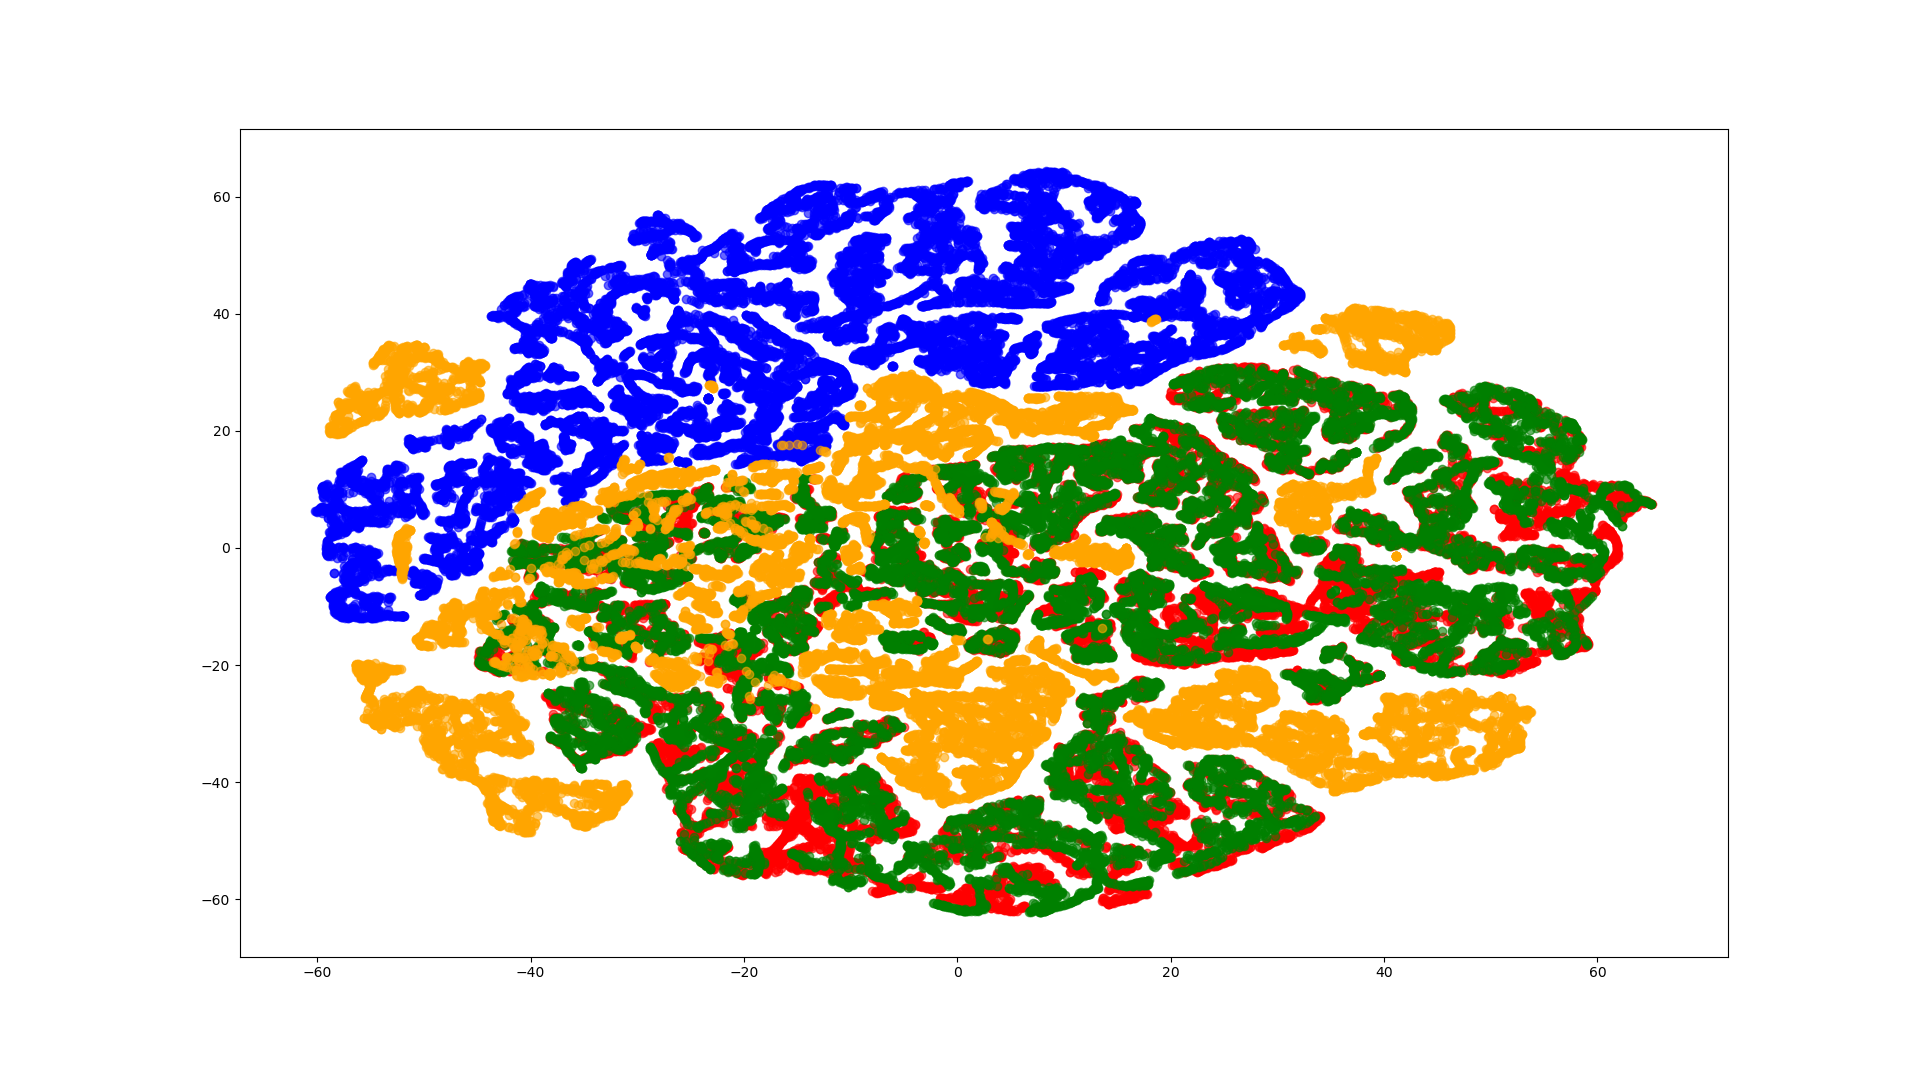
\includegraphics[width=0.60\textwidth]{../1000_TSNE_4classes.png} \\
SINGLELINES: TSNE of 4 classes, single lines. SNR 0



\end{document}